\chapter{Architecture of \libname}
\label{cha:arch}

%==============================================================================
\section{Overview}
\label{sec:arch.overview}


%==============================================================================
\section{System Requirements}
\label{sec:arch.requirements}

All design decisions and the basic structure of the \libname{ }was based on the system requirements. These requirements are:

\begin{enumerate}
	\item the library must be portable among various compilers and systems;
	\item the library must provide an easy to use framework for MAM developers;
	\item the library must be implemented using the object oriented approach;
	\item multiple instances of MAMs may exists in the same program at same time without interfering each other;
	\item the library must be easy to use and install even in existing programs;
	\item the insertion of new objects and metric distance functions must be easy even for users that do not know the details about the MAM implementation;
	\item the addition of new MAMs must be easy and all support features, such as query visualization support, must be shared among them;
	\item all MAMs must be able to store their data in memory and block devices;
	\item the storage support must be extensible to make the integration with DBMSs as simple as possible.
\end{enumerate}

All these requirements were used to create an object oriented framework which is based on three distinct layers, each one responsible for one of the basic functions: the object and metric distance functions implementations, the MAM's implementations and the storage access device implementations.

%==============================================================================
\section{Design Philosophy}
\label{sec:arch.philosophy}

As told in Section \ref{sec:arch.requirements}, the design of \libname{ } is based on its requirements. The first requirement did not affected the design of the library since it is related only to implementation issues. The rest of the requirements were decisive to define how this library will be structured.

The main idea behind the project remains on the encapsulation of each component of the library using the object oriented approach. In other words, each component must be able to manipulate its data without the interference of other components. This concept is applied to classes and group of classes related to the same function. The other important concept used was the polymorphism of the components (the ability of a component to behave according to a given interface regardless of its implementation).

The result of these concepts combined with the system requirements is a structure based on three distinct layers stacked one on top of the other. Each layer provides a set of services to the neighbor layers by using a well defined communication interface that never vary regardless of the implementation of each level. It makes possible to complain with all requirements in a easy to use and understand approach.

%==============================================================================
\section{The three layers}
\label{sec:arch.layers}

The \libname{ }is divided in three distinct layers, the User Layer, the Structure Layer and the Storage Layer, stacked one on top of the other. Each layer has a fixed communication interface which is used by other layers to request services to this layer. These interface is defined by a set of classes and interfaces which never varies regardless of the layer implementation. Figure \ref{fig:arch.layers} shows the schema of the three layers, user application and storage devices. It also shows the main classes/interfaces for each level.

\begin{figure}[tb]
	\centering
	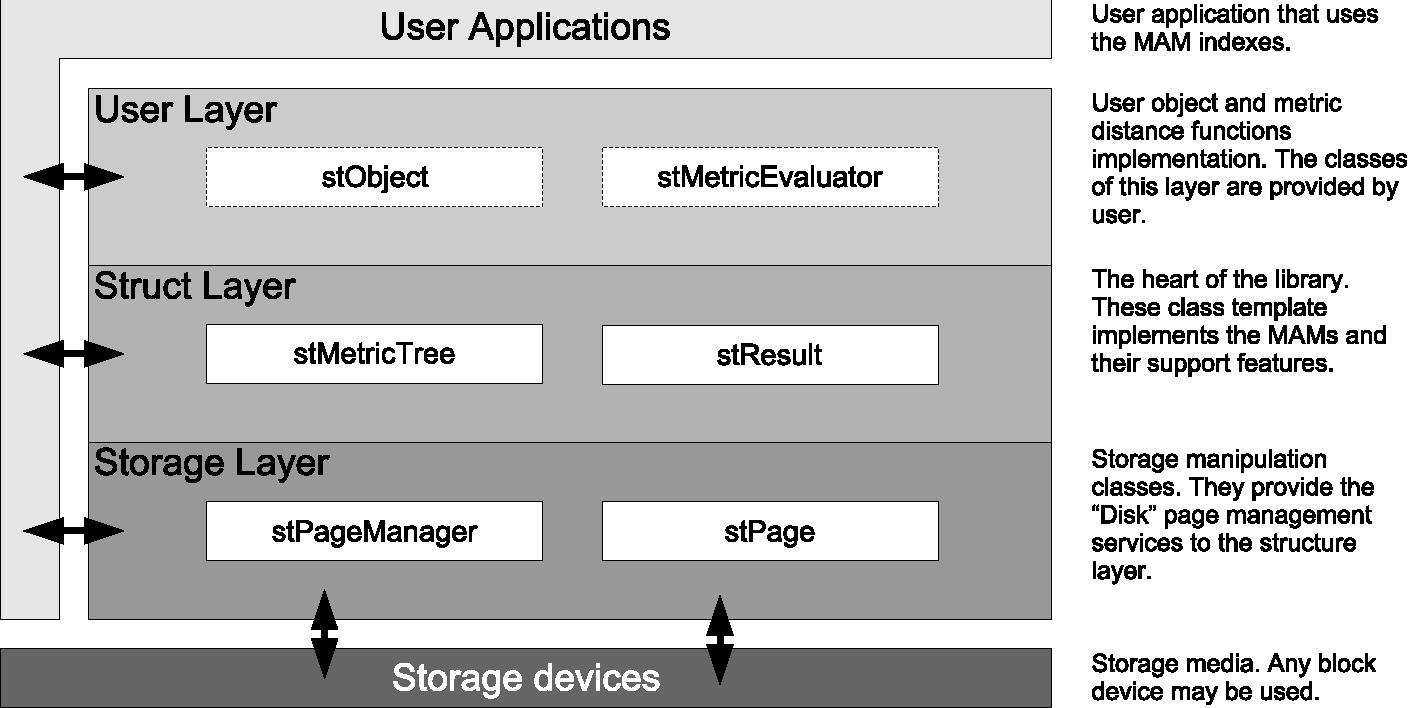
\includegraphics[width=16cm]{layers.pdf}
	\caption{The schema of the library layers and the main classes/interfaces of each layer. The dashed white boxes represent the interfaces while solid white boxes represent the classes.}
	\label{fig:arch.layers}
\end{figure}

The first layer is the {\bf User Layer} which has the knowledge of the object's nature and its metric distance functions. Since the nature of the objects may vary for each object domain, this layer is implemented by users, following a well defined interface for the objects and their metrics. This layer can only communicates with the Structure Layer and the host application.

The second layer is the {\bf Structure Layer} which implements the MAMs. It uses the User Layer classes provided by users to abstract both the object and the distance function. To store the MAM's data, it uses the storage services provided by the Storage Layer. Since this layer must support previously unknown object types, this layer is implemented with class templates and some regular classes.

The last layer is the {\bf Storage Layer} which provides the access to storage devices. The classes of this layer may be compared to ``device drivers'' since they encapsulate the storage devices to the Structure Layer. This version comes with support for both memory and disk devices but more devices may be added in future version.

These layers are summarized in the following sections and are better described by the Chapters  \ref{cha:userlayer},  \ref{cha:structurelayer} and \ref{cha:storagelayer}.

%------------------------------------------------------------------------------
\subsection{User Layer}
\label{sec:arch.user}

The User Layer abstracts the objects and their metric distance functions. It defines two class interfaces (not a class hierarchy), stObject and stMetricEvaluator, which are used by the Struct Layer to represent the indexed objects and their related metric distance function respectively.

Usually the classes of this layer are implemented by users following the definition of the stObject and stMetricEvaluator interfaces but this library provides a set of class templates which implement those interfaces for simple array and string types and a few commonly used distance functions such LEdit \cite{?} and the Lp family \cite{} distance functions. See Chapter \ref{cha:userlayer} for further details.

%------------------------------------------------------------------------------
\subsection{Structure Layer}
\label{sec:arch.struct}

The Structure Layer is the heart of the \libname. It contains the the implementations of all MAMs and their support classes. It uses the user Layer Classes to abstracts the objects and the metric distance functions and stores its data in the disk and/or memory using the services provided by the Storage Layer.

This layer defines two main class templates, the stMetricTree and the stResult. The first is the base class for all MAMs and the later is the class that encapsulates a query result. The use of the base class stMetricTree allows the applications to use all MAMs with the same basic interface. In other words, a MAM can be replaced by other without major changes in the source code.

Since this layer does not need to ``know'' the implementation of the object and the metric distance function, the addition of new objects and functions does not require modifications in this layer. See Chapter \ref{cha:structurelayer} for further details.

%------------------------------------------------------------------------------
\subsection{Storage Layer}
\label{sec:arch.storage}

The Storage Layer provides storage services to the Structure Layer. It abstracts all storage devices as a set of services that are accessible using the interface defined by the class stPageManager. So, it looks like a set of device drivers for the Structure Layer.

The idea of the stPageManager is simple, it must provide to the Structure Layer all methods necessary to manipulate a file of disk pages (the class stPage). By definition, this layer can not interact with the User Layer directly. See Chapter \ref{cha:storagelayer} for further details.

%==============================================================================
\section{Advantages and Limitations of this architecture}
\label{sec:arch.advantages}

All architectures has its advantages and limitations and \libname{ }is not an exception to this. This section will advocate the advantages and also expose the known limitations of the project of this library. The intent of expose the limitations is to allow other developers to help to improve the project and mitigate or even eliminate these limitations.

\subsection{Advantages}
\begin{enumerate}
	\item user objects and metric distance functions may be added without the knowledge of the MAM and disk access implementations;
	\item existing programs may use this library with minimum efforts to install the library to existing objects and distance functions;
	\item MAM developers may use this framework to create their MAM implementations without need to implement everything from the roots;
	\item the developers can take advantage of some development tools which are integrated to the framework such as query visualization tools and statistic support;
	\item MAM developers must provide only one generic implementation of their structures. It is not necessary to create one version for each storage device, object and metric distance function combination;
	\item some commonly used functions to perform queries are ready to use;
	\item the MAMs implemented by this library can be fairly compared since they use the same base for distance functions and disk access;
	\item each combination of object and metric distance function has its own object code (use of templates) but this approach can be easily replaced by a class hierarchy.
\end{enumerate}

\subsection{Known Limitations}
\begin{enumerate}
	\item The use of templates makes the code a little messy and hard for beginner developers;
	\item the use of distinct classes for the object and the distance functions is a quite unusual for object oriented designs;
	\item the use of classes add a little penalty to efficiency (class management overhead);
	\item the user layer is a quite difficult to understand and implement.
\end{enumerate}

%==============================================================================
\section{conclusion}
\label{sec:arch.conclusion}

This chapter describes the design issues, requirements and the basic concepts of the architecture of the \libname. It explains how the library is organized in layers and why it is organized in this way.
The existence and the arrangement of the three layer is explained as the main aspects of their interaction.

Additionally, there is a section that explains the advantages and limitations of \libname{ }which provide additional information to the understanding of the architecture and their design principles.
